\section{Experiments: discovery, residuals, and cost}
\label{sec:revision-experiments}

We test the nonradial path in Eq.~\eqref{eq:harmonic-map} with $a=0.4$, deformation amplitude $0.18$, and $T=1$. The global contraction bound is below $0.313$, so every field evaluation uses a convergent inverse-map iteration. The path, correction family, and fitted correction stay fixed as the Euler grid is refined. Results are deterministic population quadratures, except for the separately identified noisy regression experiment.

\paragraph{Correction discovery and certification.}
We eliminate the solenoidal coefficient $c$ from the exact residual formula in Proposition~\ref{prop:harmonic-search}, enumerate every real root of the remaining quartic's derivative, and evaluate the original sum of squares at each root. This recovers $(\omega,c)=(0.4,0.32)$ to floating-point precision without initializing at the solution. The coefficient identity in the proposition certifies the exact zero; the approximately $2.1\times10^{-16}$ numerical residual is a floating-point evaluation, not an interval enclosure. A local least-squares run started at $\omega=-0.3$ instead converges to $\omega\simeq-0.392394$, with residual upper bound $0.07241$. Thus a successful local optimization termination does not establish feasibility. Global enumeration takes about $0.01$ seconds including three local comparison runs.

\paragraph{Distribution and particle errors.}
Figure~\ref{fig:revision-convergence} reports the second-moment lower bound and the rotation-coupling upper bound from Theorem~\ref{thm:harmonic-coupling}. We evaluate these continuum bounds by $64$-point radial Gauss--Laguerre quadrature and $64$ equally spaced angles. They are not exact evaluations of $W_2$, and the quadrature is not interval certified. At $N=512$, corrected Euler gives bounds $3.439\times10^{-7}$ and $4.881\times10^{-7}$, with observed orders $1.9983$ and $1.9992$ from $N=256$ to $512$. Its common-start particle error is $6.609\times10^{-4}$, with order $0.9992$. Base Euler's lower and upper bounds both have order $0.9991$. Refining to $96$ radial nodes and $128$ angles changes the corrected upper bound by less than $8\times10^{-17}$. Independent DOP853 trajectories at four intermediate times agree with the analytic flows within $6.5\times10^{-12}$ on the tested labels. These checks support the exact path-preservation identity; they do not replace it.

\begin{figure*}[t]
\centering
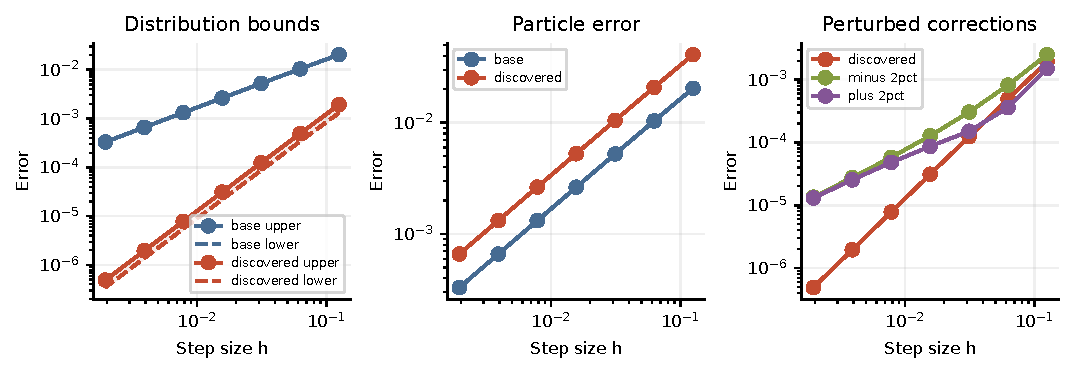
\includegraphics[width=\textwidth]{../results/revision/harmonic_convergence.pdf}
\caption{Nonradial correction discovery followed by fixed-field refinement. Left: quadrature evaluations of lower and upper bounds on full $W_2$, with the region between them shaded. Center: common-start particle RMS. Right: fixed $2\%$ perturbations of the discovered rotation restore an approximately first-order distribution-error trend. The corrected upper bound uses measure-preserving label rotation, not a same-start particle comparison.}
\label{fig:revision-convergence}
\end{figure*}

\paragraph{Residuals, infeasibility, and model error.}
Changing $\omega$ by $-2\%$ or $+2\%$ gives exact residual upper certificates $0.01345$ and $0.01372$ at $T$, and the finest observed upper-bound orders become $1.036$ and $0.961$. On the infeasible Gaussian path $\Sigma_t=\operatorname{diag}(1+t,1+t+2t^2)$, the scalar energy budget is positive throughout $[0,1]$, whereas the first coordinate gives the all-field lower bound $\varepsilon_t\ge[4(1+t)^{3/2}]^{-1}$. A separate one-coefficient noisy velocity regression over three seeds has analytically known learned paths. Refining Euler reduces its integration error while target error approaches the nonzero continuous-path error. This is a restricted parametric learning check, not a neural generative-model benchmark.

\paragraph{Cost and unfavorable baselines.}
Table~\ref{tab:revision-cost} preserves the comparison at $384$ field evaluations. Heun's evaluated upper bound is slightly below corrected Euler's evaluated lower bound, providing numerical evidence that Heun is more accurate on this path. RK3 is substantially better. Batch runtimes are comparable, and every stage pays for the inverse map; no sampling speedup is established. The correction improves Euler's distribution order, but it is not the best solver in this experiment. Supplement Section~\ref{sec:revision-experiments-details} gives timings, inverse tolerances, refinement data, optimizer failures, model-error floors, and reproduction commands.

\begin{table}[t]
\centering
\caption{Nonradial path at equal $384$ field evaluations. These are quadrature evaluations of continuum $W_2$ bounds.}
\label{tab:revision-cost}
\scriptsize
\begin{tabular}{@{}lrrr@{}}
\toprule
Method & $W_2$ lower & $W_2$ upper & Particle RMS\\
\midrule
Corrected Euler & $6.111\times10^{-7}$ & $8.675\times10^{-7}$ & $8.810\times10^{-4}$\\
Base Heun & $6.073\times10^{-7}$ & $6.085\times10^{-7}$ & $6.085\times10^{-7}$\\
Base RK3 & $1.067\times10^{-9}$ & $1.070\times10^{-9}$ & $1.070\times10^{-9}$\\
\bottomrule
\end{tabular}

\end{table}
